\section{Verhaltensdarstellung über Komplexe Zahlen}
Normalerweise werden komplexe Zahlen via der imaginären Einheit $\imu^2 \coloneqq -1$ eingeführt.
Anschließend definiert man dann die komplexen Zahlen über $\mathbb{C} \ni c \coloneqq a + b\cdot \imu$ mit $a,b \in \mathbb{R}$.
Aus dieser Herangehensweise folgen dann recht schnell die Regeln zum Rechnen mit ebendiesen.
\begin{align*}
    c_1 +c_2 &= (a_1 + b_1\cdot \imu) + (a_2 + b_2\cdot \imu) &
    c_1 \cdot c_2 &= (a_1 + b_1\cdot \imu) \cdot (a_2 + b_2\cdot \imu) \\
        &= (a_1 + a_2) + (b_1 + b_2)\cdot \imu  &
        &= a_1a_2 + b_1b_2 \cdot \imu^2 + a_1b_2 \cdot \imu + a_2b_1 \cdot \imu\\
        &&&= (a_1a_2 - b_1b_2) + (a_1b_2 + a_1b_2) \cdot \imu
\end{align*}

\begin{wrapfigure}{r}{0.4\textwidth}
  \begin{centering}
    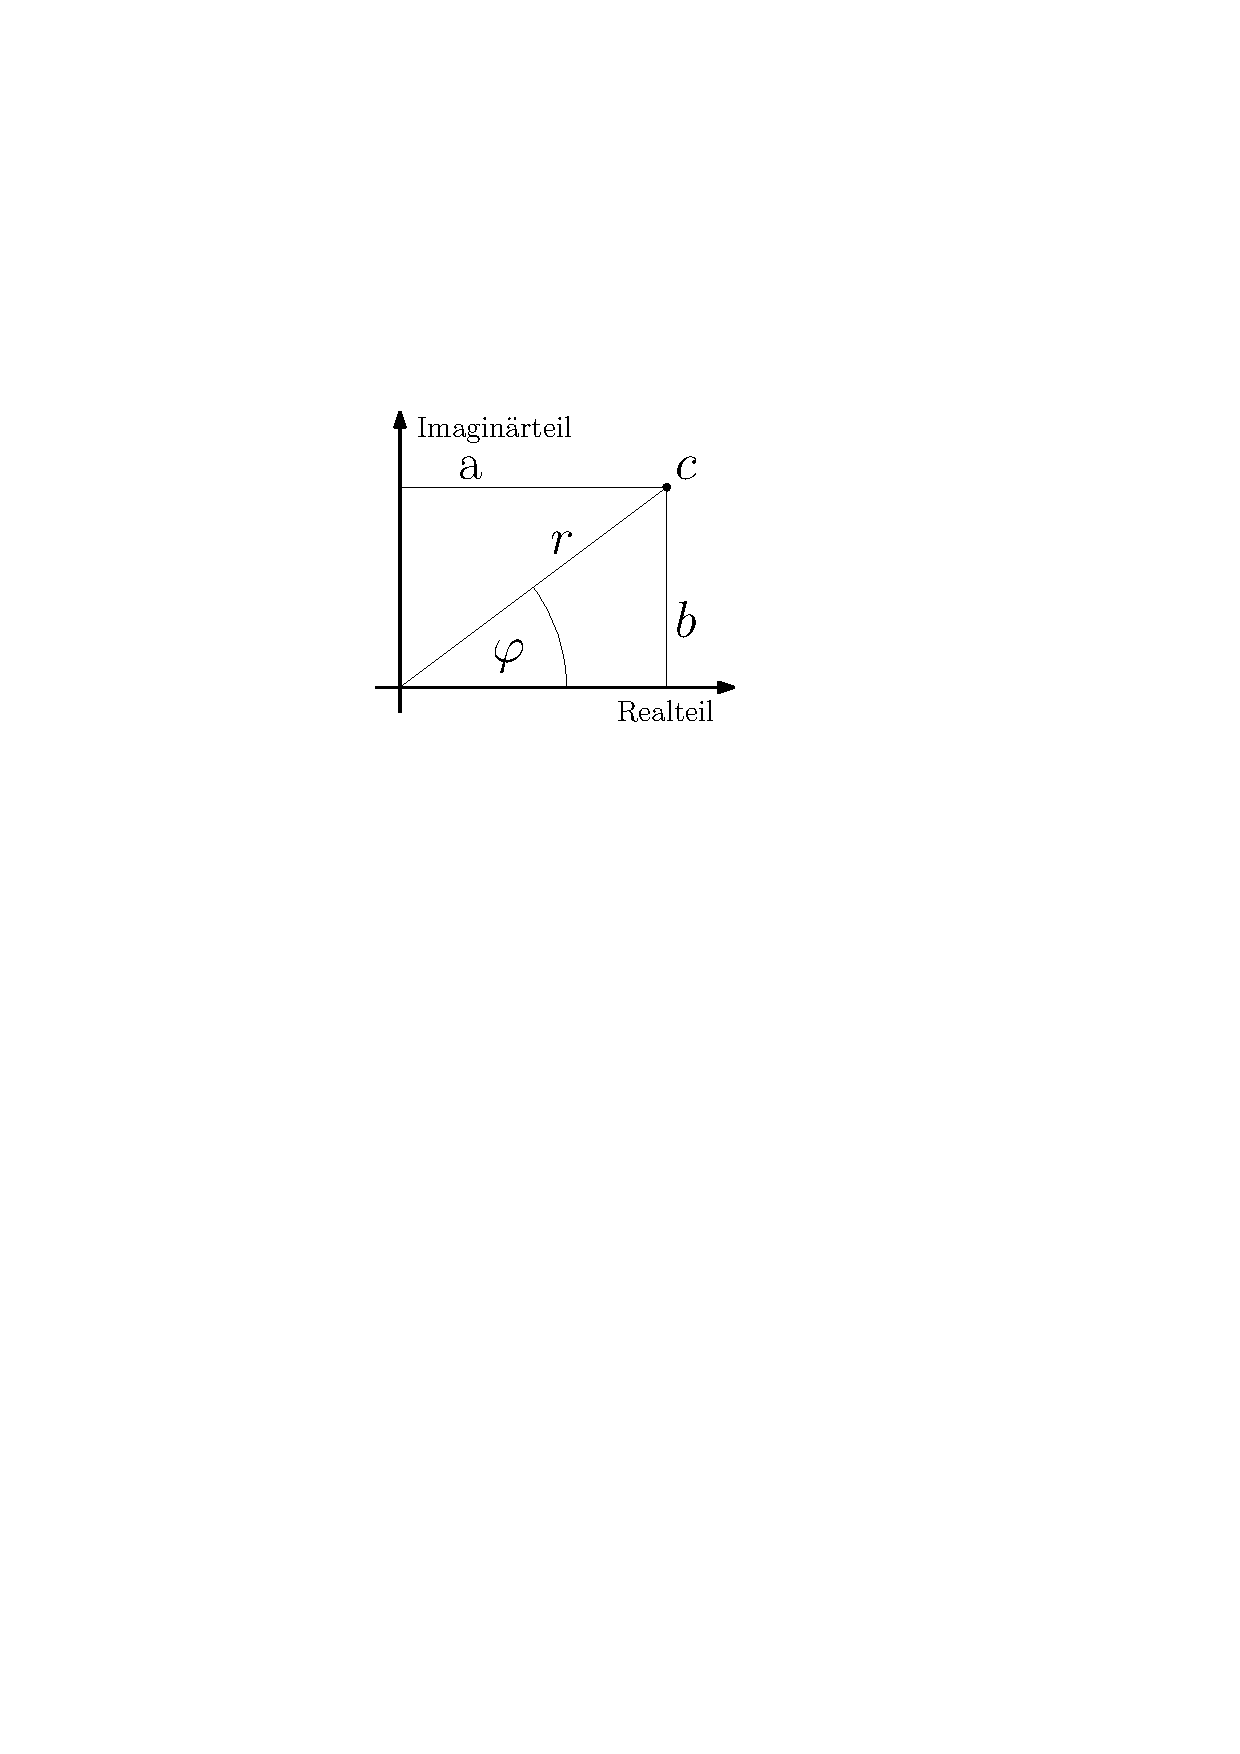
\includegraphics[width=0.4\textwidth]{philip1.pdf}
  \end{centering}
  \caption{Komplexe Zahl $c$ in kartesischen und polaren Koordinaten}
\end{wrapfigure}

Für den Anwendungsbereich der Wechselstromberechnungen ist es jedoch sinnvoller, komplexe Zahlen als
Repräsentanten von Punkten im zweidimensionalen Raum zu sehen, welche über die oben genannten Rechenvorschriften nützliche Eigenschaften besitzen, auf die im folgenden eingegangen werden soll.

Man denke sich eine komplexe Zahl $a +b\imu$ als einen Vektor $(a,\,b)_{x,y}$ im kartesischen Koordinatensystem mit X- und Y-Achse.
Dann sieht man, dass die Addition zweier komplexer Zahlen genau der Vektoraddition entspricht.
Weiterhin kann man den Vektor auch in einem polaren Koordinatensystem darstellen, in dem man aus $a$ und $b$ den 
Abstand zum Koordinatenursprung $r$ und den Winkel zur X-Achse $\varphi$ berechnet. Diese Form führt zu einer deutlich einprägsameren Multiplikationsformel.  
\begin{align*}
    a&=r \cdot \cos(\varphi) & c_1 &= a_1+b_1\imu = r_1\cos(\varphi_1) + r_1\sin(\varphi_1)\imu  \\
    b&=r \cdot \sin(\varphi) & c_2 &= a_2+b_2\imu = r_2\cos(\varphi_2) + r_2\sin(\varphi_2)\imu
\end{align*} \vspace*{-5mm}
\begin{align*}
    c_1 \cdot c_2 &= (r_1r_2\cos(\varphi_1)\cos(\varphi_2) - r_1r_2\sin(\varphi_1)\sin(\varphi_2)) \\
    &\quad + (r_1r_2\cos(\varphi_1)\sin(\varphi_2) + r_1r_2\cos(\varphi_2)\sin(\varphi_1)) \cdot \imu\\
    &= r_1r_2 \cdot \big(\cos(\varphi_1 + \varphi_2) + \sin(\varphi_1 + \varphi_2)\imu\, \big)
\end{align*} \vspace*{-5mm}
\begin{align*}
    (r_1,\varphi_1)_{r,\,\varphi} \cdot (r_2,\,\varphi_2)_{r,\varphi} = (r_1 \cdot r_2,\, \varphi_1 + \varphi_2)_{r,\varphi}
\end{align*}
Die Multiplikation zweier solcher Vektoren dreht den ersten also noch um den Winkel des zweiten weiter, und streckt die Länge $r_1$ um den Faktor $r_2$

Um nun zu verstehen, wie komplexe Zahlen 
bei der Berechnung der Interaktion von passiven elektrischen Bauteilen mit dem eingehenden Spannungs- oder Stromsignal helfen, stellen wir sowohl Signal als auch Bauteil als (polare) komplexe Zahl dar.

\subsection{Signal}
Das Signal sei eine harmonische Kosinusschwingung mit Frequenz (Kreisfrequenz $\omega$), Amplitude $A$ und Ausgangsphase $\phi_0$ .
Wir stellen dies als einen kreisförmig um den Koordinatenursprung oszillierenden Punkt $P$ dar.
$$P = (A \cos(\omega t + \phi_0), A \sin(\omega t + \phi_0))_{x,y} = (A,\omega t + \phi_0)_{r,\,\varphi}$$
Der Winkel zur X-Achse ist dabei genau die Phase zum Zeitpunkt $t$, der Abstand zum Ursprung die Amplitude, und die Projektion auf die X-Achse den Wert der Schwingung zum Zeitpunkt $t$.

Eine plötzliche Phasenänderung würde den Punkt auf seiner Bahn nach vorn oder zurück springen lassen, und eine Änderung der Schwingungsamplitude würde den Bahnradius verändern.

Eine solche Bahn lässt sich im komplexen leicht durch eine Exponentialfunktion
ausdrücken. Deswegen wird eine harmonische Schwingung in der komplexen Wechselstromrechnung durch diese beschrieben.
$$A e^{\imu \omega t + \imu \phi_0} = A\cos(\omega t + \phi_0) + A\sin(\omega t + \phi_0)\imu = (A,\omega t + \phi_0)_{r,\,\varphi}$$


\subsection{Impendanz}
This is more testing text.
